\documentclass[10pt, a4paper]{report}

\pdfpagewidth\paperwidth
\pdfpageheight\paperheight

\usepackage[utf8]{inputenc}
\usepackage[T1]{fontenc}
\usepackage[italian]{babel}
\usepackage{mathtools, amsmath, amssymb, amsthm}
\usepackage[hidelinks]{hyperref}
\usepackage{graphicx, tikz}
\usepackage{xcolor, listings}

\definecolor{background_color}{rgb}{0.9, 0.9, 0.9}
\definecolor{keyword_color}{rgb}{0.2, 0.4, 0.8}
\definecolor{comment_color}{rgb}{0.5, 0.5, 0.5}
\definecolor{string_color}{rgb}{0.8, 0.7, 0.2}
\definecolor{lightgray}{rgb}{0.95, 0.95, 0.95}
\definecolor{darkgray}{rgb}{0.4, 0.4, 0.4}
\definecolor{editorGray}{rgb}{0.95, 0.95, 0.95}
\definecolor{editorOcher}{rgb}{1, 0.5, 0}
\definecolor{editorGreen}{rgb}{0, 0.5, 0}
\definecolor{orange}{rgb}{1,0.45,0.13}
\definecolor{olive}{rgb}{0.17,0.59,0.20}
\definecolor{brown}{rgb}{0.69,0.31,0.31}
\definecolor{purple}{rgb}{0.38,0.18,0.81}
\definecolor{lightblue}{rgb}{0.1,0.57,0.7}
\definecolor{lightred}{rgb}{1,0.4,0.5}

\lstdefinelanguage{HTML5}{
	language=html,
	sensitive=true,
	alsoletter={<>=-},
	morecomment=[s]{<!-}{-->},
	tag=[s],
	otherkeywords={
			% Standard tags
			!DOCTYPE, html, head, title, style, link, meta, body,
			% Divs
			div,
			% scripts
			script,
			% More tags...
			canvas, svg, rect, animateTransform, video, source, iframe,
			image, header, article
		}
}

\lstdefinestyle{html} {
	% General design
	backgroundcolor=\color{editorGray},
	basicstyle={\small\ttfamily},
	frame=single,
	% line-numbers
	numbers=left,
	stepnumber=1,
	firstnumber=1,
	numberfirstline=true,
	% Code design
	identifierstyle=\color{black},
	keywordstyle=\color{blue}\bfseries,
	ndkeywordstyle=\color{black}\bfseries,
	stringstyle=\color{editorOcher}\ttfamily,
	commentstyle=\color{brown}\ttfamily,
	% Code
	language=HTML5,
	alsodigit={.:;},
	tabsize=4,
	showtabs=false,
	showspaces=false,
	showstringspaces=false,
	extendedchars=true,
	breaklines=true,
}

% JavaScript
\lstdefinelanguage{JavaScript}{
	morekeywords={
		typeof, new, true, false, catch, function, return, null, catch, switch,
		var, if, in, while, do, else, case, break
	},
	morecomment=[s]{/*}{*/},
	morecomment=[l]//,
	morestring=[b]",
	morestring=[b]',
	morestring=[b]`
}

\lstdefinestyle{js} {
	% General design
	backgroundcolor=\color{editorGray},
	basicstyle={\small\ttfamily},
	frame=single,
	% line-numbers
	numbers=left,
	stepnumber=1,
	firstnumber=1,
	numberfirstline=true,
	% Code design
	identifierstyle=\color{black},
	keywordstyle=\color{blue}\bfseries,
	ndkeywordstyle=\color{lightblue}\bfseries,
	stringstyle=\color{editorOcher}\ttfamily,
	commentstyle=\color{brown}\ttfamily,
	% Code
	language=JavaScript,
	alsodigit={.:;},
	tabsize=4,
	showtabs=false,
	showspaces=false,
	showstringspaces=false,
	extendedchars=true,
	breaklines=true,
}

\title{Computer Grafica}
\author{Federico Bustaffa}
\date{17/02/2022}

\begin{document}

\maketitle
\tableofcontents

% capitolo 1
\part{Matematica e teoria}\label{matematica}
Questa prima parte tratter\`a unicamente la teoria necessaria a comprendere la parte successiva, nella quale invece
si avr\`a un approccio pi\`u pratico. Nella parte successiva vedremo il codice Javascript necessario alla costruzione
di un ambiente grafico utilizzando l'API OpenGL. Nello specifico verr\`a utilizzata WebGL ovvero la versione OpenGL
per applicazioni Web.

\chapter{Colori}\label{colori}
In questo primo capitolo verr\`a trattato il colore e come esso pu\`o essere manipolato.

\section{Fisica e percezione dei colori}
Il colore che noi percepiamo dipende da due fattori: \textbf{fisico} e \textbf{}.
L'aspetto fisico riguarda il come la luce rimbalza sull'oggetto e poi arriva al
nostro occhio. L'aspetto percettivo riguarda il come il nostro occhio elabora la
luce che arriva produce di conseguenza un colore.

\section{Luce come fenomeno ondulatorio}
La luce come fenomeno ondulatorio \`e caratterizzata da due fattori:
\begin{itemize}
	\item \textbf{Ampiezza}: il valore del picco di ogni onda.
	\item \textbf{Lunghezza d'onda}: la distanza tra due picchi consecutivi. Inversamente
	      proporzionale alla lunghezza d'onda \`e la \textbf{frequenza}: pi\`u i picchi sono
	      vicini pi\`u la frequenza \`e alta. La frequenza si pu\`o ottenere con la formula:
	      \[ f = \frac{c}{l} \]
	      dove $c$ \`e la velocit\`a della luce e $l$ \`e la lunghezza d'onda.
\end{itemize}
Lo spettro della luce visibile ha questo range di lunghezze d'onda

\begin{center}
	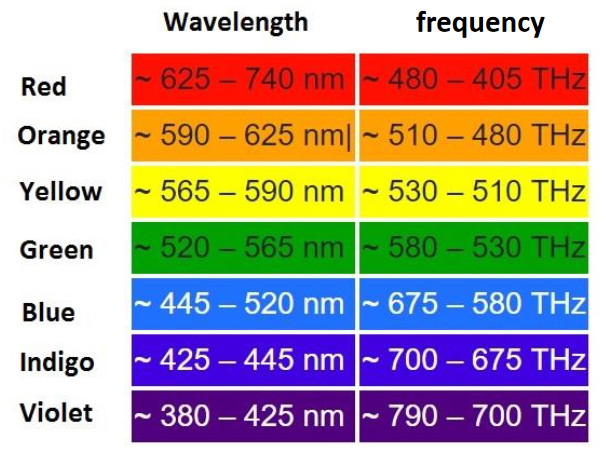
\includegraphics[width=0.5\textwidth]{immagini/spettro_visibile}
\end{center}

\section{Luce come insieme di particelle}
La luce \`e fatta di fotoni, particelle senza massa che viaggiano alla velocit\`a della luce.
Un fascio di luce \`e un insieme di fotoni, ciascuno con la propria frequenza, energia e
colore. Il colore del fascio di luce dipende da come l'insieme di fotoni \`e distribuito sullo
spettro delle frequenze. A noi interessa in particolare questo modo di vedere la luce.

\section{Percezione del colore}
Gli oggetti non hanno un colore, hanno delle propriet\`a fisiche e la luce viene riflessa in
base
\begin{itemize}
	\item alle propriet\`a dei materiali di cui \`e composto l'oggetto.
	\item alle caratteristiche della luce.
	\item al colore intorno all'oggetto.
	\item alla percezione dell'osservatore.
\end{itemize}
La nostra percezione della luce \`e \textbf{additiva}. Se ho quindi due luci di colore diverso
che si sovrappongono vedo la combinazione delle due. Se ho tutti e tre i colori primari insieme
vedo una luce bianca.

Noi vediamo meglio la luce con lunghezza d'onda intorno ai 550nm, ovvero vediamo questi colori
come pi\`u luminosi. La \textbf{funzione di efficienza luminosa fotopica} ce lo mostra.
\begin{center}
	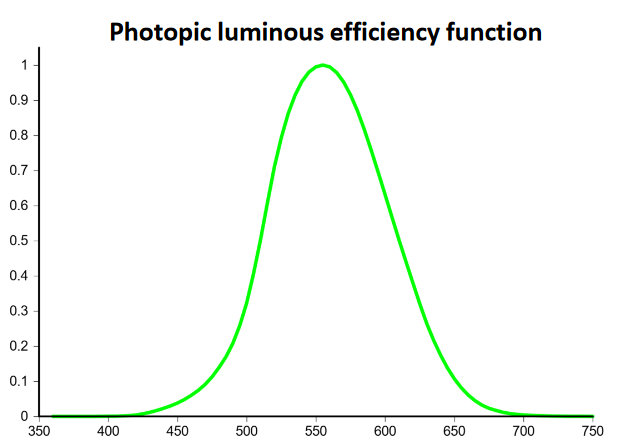
\includegraphics[width=0.5\textwidth]{immagini/funzione_fotopica}
\end{center}
Se ho una luce, per sapere come la percepisco, la moltiplico in ogni punto per la funzione
fotopica.

\section{Coefficienti tricromatici e valori RGB}
Se io dovessi regolare tre manopole, una che regola l'intenst\`a del rosso, una del verde e
una del blu e volessi ottenere una luce bianca alla fine avrei tre valori diversi per ogni
manopola, diciamo $r, g, b$. Quello che vogliamo, per\`o, \`e che il bianco, che \`e la somma
di tutti i colori, sia effettivamente rappresentato come combinazione dei tre colori (rosso,
verde e blu) ognuno col massimo valore e soprattutto vogliamo che questo valore sia uguale
per tutti e 3 i colori. Non devono perci\`o dipendere dalla nostra percezione.

Se volessi rappresentare il tutto con un'equazione sarebbe cos\`i.
\[ Bianco = r \cdot m_r \oplus g \cdot m_g \oplus b \cdot m_b \]
dove $a \oplus b$ indica la percezione delle luci $a$ e $b$ sovrapposte e dove
$m_r, m_g, m_b$ sono delle costanti che valgono
\[ m_r = 1 \quad m_g = 4.39 \quad m_b = 0.0048 \]
l'obbiettivo \`e quello di ottenere
\[ r \cdot m_r = g \cdot m_g = b \cdot m_b \]
Ecco che entrano in gioco i \textbf{coefficienti tricromatici} definiti come segue
\begin{gather*}
	\alpha = \frac{r \cdot m_r}{r \cdot m_r + g \cdot m_g + b \cdot m_b} \\
	\\
	\beta = \frac{g \cdot m_g}{r \cdot m_r + g \cdot m_g + b \cdot m_b} \\
	\\
	\gamma = \frac{b \cdot m_b}{r \cdot m_r + g \cdot m_g + b \cdot m_b}
\end{gather*}
A questo punto ho che il generico colore $C$ \`e dato da
\[ C = \alpha \oplus \beta \oplus \gamma \]
vale inoltre che
\[ \alpha + \beta + \gamma = 1 \]
Questo procedimento ha come risultato quello di non considerare la \emph{luminanza} e tenere
di conto solo la mistura di colori nella stessa misura per ogni primario.

Se volessimo invece ottenere la luminanza di un certo colore, sapendo i suoi coefficienti
tricromatici dovremmo calcolare
\[ L = \alpha \cdot m_r + \beta \cdot m_g + \gamma \cdot m_b \]

Ma come facciamo a ottenere i valori RGB di un colore non spettrale ?
Dobbiamo sapere quanto rosso, quanto verde e quanto blu mettere. La "quantit\`a" di colore che
dobbiamo mettere \`e data dalle seguenti sommatorie
\begin{gather*}
	R = \sum_{\lambda = 380}^{\lambda = 780} \overline{r}(\lambda) E(\lambda) \\
	\\
	G = \sum_{\lambda = 380}^{\lambda = 780} \overline{g}(\lambda) E(\lambda) \\
	\\
	B = \sum_{\lambda = 380}^{\lambda = 780} \overline{b}(\lambda) E(\lambda) \\
\end{gather*}
Dove le funzioni soprasegnate sono la \emph{color matching function} dello specifico colore,
ovvero quanto di quel colore vedo ad una determinata frequenza della luce, nel punto
$\lambda$ mentre $E(\lambda)$ equivale all'energia che arriva nello spettro.

\section{Spazi di colori}
Per ottenere sfumature di colore in modo pi\`u agevole sono stati introdotti
degli \textbf{spazi di colori}.

\subsection{HSV}
L'HSV (\textbf Hue, \textbf Saturation and \textbf Value) funziona in questo modo:
\begin{itemize}
	\item Il primo valore \`e la tinta, il colore scelto.
	\item Il secondo valore \`e la saturazione e l'idea \`e quella di impostare con essa,
	      quanto grigio si vuole aggiungere al colore scelto. Se la saturazione \`e
	      massima non aggiunger\`o grigio al mio colore, se \`e minima otterr\`o proprio
	      il grigio. Il valore minimo \`e 0 e il valore massimo \`e 1 ma questi valori
	      dipendono in modo proporzionale dal prossimo valore.
	\item Il terzo valore \`e la luminosit\`a del grigio che sto aggiungendo al mio colore.
	      Con il valore massimo otterr\`o il bianco, con il minimo otterr\`o il nero
	      (valore minimo 0, valore massimo 1).
\end{itemize}

\subsection{HSL}
L'HSL (\textbf Hue, \textbf Saturation and \textbf Lightness) molto simile al precedente. In
questo caso abbiamo il valore della \textbf{luminosit\`a} che va da $-0.5$ a $0.5$ in questo
caso la saturazione \`e massima con luminosit\`a 0 e si abbassa se la luminosit\`a cala o
incrementa.

% capitolo 2
\part{Calcolabilità}

\chapter{Introduzione alla calcolabilità}
Iniziamo con la \textbf{teoria della calcolabilità} la quale
si pone come obbiettivo quello di definire cosa siano problemi,
funzioni e algoritmi, cercando di dare una definizione formale
di questi ultimi. Una volta definiti questi concetti sarà di
nostro interesse capire quali sono i problemi
\textbf{calcolabili} e quali invece no.

In questa prima parte non è di nostro interesse tenere di conto
le limitazioni che hanno i calcolatori reali. Ragioneremo quindi
supponendo che non questi non abbiamo limiti in tempo o spazio
per effettuare il calcolo.

Cercheremo quindi di capire quali sono i problemi
\textbf{calcolabili} mediante una \textbf{procedura effettiva},
quali invece \textbf{non} sono calcolabili per capire se ce ne
sono di interessanti, se ne esistono di reali o se sono solo
artificiali e puramente teorici.

\section{Disegnare un triangolo}
L'obbiettivo per il momento \`e disegnare un triangolo di questo tipo:
\begin{center}
	\begin{tikzpicture}[scale=2.5]
		\draw[->, dashed]
		(-1.0, 0) node[above] {-1.0}
		--
		(1.0, 0) node[above] {1.0} node[below] {$x$};
		\draw[->, dashed]
		(0, -1) node[right] {-1.0}
		--
		(0, 1) node[right] {1.0} node[left] {$y$};
		\filldraw[color=red, fill=red!60, very thick]
		(-0.5, -0.5) node[left, color=black] {(-0.5, -0.5)}
		--
		(0, 0.5) node[right, color=black] {(0.0, 0.5)}
		--
		(0.5, -0.5) node[right, color=black] {(0.5, -0.5)}
		--
		cycle;
	\end{tikzpicture}
\end{center}

\subsection{Array Buffer}
Per iniziare a disegnare qualcosa dobbiamo dare a WebGL delle informazioni sulla geometria
che vogliamo visualizzare.

Se volessimo disegnare un triangolo, la prima cosa che probabilmente ci verr\`a in mente
\`e specificare le coordinate $(x, y)$ dei tre vertici.

Iniziamo con il definire un array di \emph{float} contenente i nostri vertici.
\begin{lstlisting}[style=js]
function geometrySetup() {
	var data = new Float32Array([
		-0.5, -0.5,
		 0.0,  0.5,
		 0.5, -0.5
	]);
\end{lstlisting}
Ora vogliamo rendere questi valori visibili dalla scheda grafica. Per farlo dobbiamo metterli
in un \textbf{buffer} da cui poi verranno letti.
\begin{lstlisting}[style=js, firstnumber=7]
	var buffer = gl.createBuffer();
	gl.bindbuffer(gl.ARRAY_BUFFER, buffer);
	gl.bufferData(gl.ARRAY_BUFFER, data, gl.STATIC_DRAW);
\end{lstlisting}
Spieghiamo queste 3 righe di codice:
\begin{enumerate}
	\item Viene creato un buffer nella memoria della GPU.
	\item Il buffer viene associato a un target (in questo caso \emph{ARRAY\_BUFFER}).
	\item I dati dell'array \emph{data} vengono caricati nel buffer.

	      L'ultimo parametro \`e un
	      suggerimento che per l'ottimizzazione. In questo caso ci dice che i dati caricati
	      nel buffer non dovrebbero variare molto. Nel caso in cui volessimo disegnare
	      qualcosa in movimento potrebbe essere una buona scelta usare \emph{DYNAMIC\_DRAW}.
\end{enumerate}

\subsection{Vertex Attribute Array}
Ora per\`o dobbiamo dire al programma come leggere questi dati.
Per prima cosa dobbiamo sapere che ogni scheda video ha in memoria una sorta array in
cui si possono inserire le "\emph{istruzioni}" su come leggere i dati che abbiamo caricato
precedentemente nel buffer. Supponendo di averne $N$, allora saranno numerati da 0 a $N-1$
($N$ dipende dalla GPU).

In ciascuna cella dell'array sono presenti informazioni sui diversi attributi che pu\`o
avere ogni vertice della geometria che disegnamo. In questo caso abbiamo solo la posizione
del vertice ma in futuro potremo inserire anche altri attributi come ad esempio il colore.

Per il momenti limitiamoci a scrivere una cosa di questo tipo:
\begin{lstlisting}[style=js, firstnumber=10]
	gl.enableVertexAttribArray(0);
	gl.vertexAttribPointer(0, 2, gl.FLOAT, false, 8, 0);
}
\end{lstlisting}
La seconda funzione va a scrivere le informazioni necessarie a interpretare i dati nel
buffer.
\begin{itemize}
	\item Per prima cosa indichiamo in quale \textbf{posizione} dell'array degli attributi
	      vogliamo scrivere le informazioni. In questo caso 0.
	\item Il secondo parametro ci dice quanti valori devo considerare (per ciascun vertice)
	      per poter descrivere l'attributo. In questo caso abbiamo 2 dato che l'attributo
	      che vogliamo descrivere \`e la posizione del vertice (coppia $(x, y)$ di
	      coordinate).
	\item Il terzo parametro \`e semplicemente il \textbf{tipo} dei singoli valori dell'array.
	      Nel nostro caso abbiamo un array di float quindi scriviamo \emph{gl.FLOAT}.
	\item Il quarto parametro \`e la \textbf{normalizzazione} ma la vedremo pi\`u avanti.
	      Per ora lasciamolo a \emph{false}.
	\item Il quinto parametro \`e la \textbf{stride}. Indica il numero di byte che intercorre
	      tra i dati che descrivono un vertice e quello successivo. In sostanza ci dice ogni
	      quanti byte inizia la descrizione di un nuovo vertice. Nel nostro caso abbiamo 8
	      come valore perch\'e abbiamo che un vertice \`e descritto solamente dalle sue
	      coordinate spaziali $x, y$. Sono di tipo float e quindi ottengo $2 * 4 = 8$ byte
	      che dividono l'inizio di un vertice dall'altro.
	\item L'ultmo valore \`e l'\textbf{offset}. Indica quanti byte saltare prima di iniziare
	      a leggere l'array. Nel nostro caso vale 0 perch\'e iniziamo a leggere l'array
	      dall'inizio. Pi\`u avanti sar\`a utile impostare valori diversi dell'offset
	      nel caso avessimo pi\`u attributi per uno stesso vertice.
\end{itemize}
La prima funzione non fa altro che abilitare il primo slot dell'array degli attributi.
Stiamo quindi notificando il programma che al posto 0 dell'array ci sono informazioni
necessarie per interpretare i dati scritti nel buffer.

\subsection{Shader}
Ora che abbiamo comunicato alla GPU come leggere i dati nel buffer dobbiamo dargli un
metodo per disegnare la geometria che vogliamo. Per farlo utilizziamo gli \textbf{shader}.
Per scriverli si usa un linguaggio (GLSL) simile al C.

Uno shader \`e un piccolo programma che viene eseguito nella memoria della GPU ed \`e
fondamentale per la costruzione della geometria e per la fase di rendering finale.

Gli shader possono essere di due tipi: \textbf{vertex} e \textbf{fragment}.

\subsubsection{Vertex Shader}
Il vertex shader si occupa di assemblare la geometria che vogliamo disegnare.
\begin{lstlisting}[style=js]
function shaderSetup() {
	var vs_source =
		`attribute vec2 aPosition;
		
		void main()
		{
			gl_Position = vec4(aPosition, 0.0, 1.0);
		}`
	;
\end{lstlisting}
La variabile \emph{aPosition} ha due tipi: \textbf{attribute} e \textbf{vec2}. Il primo
indica che il valore deve essere preso dall'array degli attributi visto in precedenza
(dopo vediamo come fare nello specifico). Il secondo tipo indica semplicemente che
si tratta di una coppia di valori o vettore bidimensionale.

Nel \emph{main} \`e presente la variabile \emph{gl\_Position}, una variabile speciale, che
indica la posizione di ci\`o che sto disegnando.

\subsubsection{Fragment Shader}
Il fragment shader si occupa della fase di rasterizzazione, in cui si va a decidere il
colore di ci\`o che viene visualizzato.
\begin{lstlisting}[style=js, firstnumber=8]
	var fs_source =
		`void main()
		{
			gl_FragColor = vec4(1.0, 0.0, 0.0, 1.0);
		}`
	;
\end{lstlisting}
In questo caso abbiamo solo la variabile \emph{gl\_FragColor} un vettore a 4 dimensioni.
I primi 3 valori sono i valori di rosso, verde e blu, il quarto valore \`e la trasparenza.
Tutti e quattro i valori vanno da 0 a 1. Dato che abbiamo il rosso a 1, mentre il verde e
il blu sono a 0, ci aspettiamo di vedere un triangolo rosso.

\subsubsection{Compilazione}
Compiliamo i sorgenti.
\begin{lstlisting}[style=js, firstnumber=14]
	var vertex = gl.createShader(gl.VERTEX_SHADER);
	gl.shaderSource(vertex, vs_source);
	gl.compileShader(vertex);

	var fragment = gl.createShader(gl.FRAGMENT_SHADER);
	gl.shaderSource(fragment, fs_shader);
	gl.compileShader(fragment);
\end{lstlisting}
\newpage
Adesso dobbiamo linkare il tutto in unico programma.
\begin{lstlisting}[style=js, firstnumber=21]
	var program = gl.createProgram();
	gl.attachShader(program, vertex);
	gl.attachShader(program, fragment);
	gl.linkProgram(program);
	gl.useProgram(program);
\end{lstlisting}
Concludiamo con questo comando
\begin{lstlisting}[style=js, firstnumber=26]
	gl.bindAttribLocation(program, 0, "aPosition");
}
\end{lstlisting}
il quale indica allo shader di prendere le informazioni dalla posizione 0 dell'array degli
attributi e metterle dentro la variabile \emph{aPosition} del vertex shader. In questo caso
si tratta delle coordinate dei vertici del triangolo.

\section{Draw}
Non ci rimane che invocare le funzioni necessarie per disegnare il nostro triangolo rosso.
\begin{lstlisting}[style=js]
function drawTriangle() {
	gl.clearColor(1.0, 1.0, 1.0, 1.0);
	gl.clear(COLOR_BUFFER_BIT);
	gl.drawArrays(gl.TRIANGLES, 0, 3);
}
\end{lstlisting}
Le prime due funzioni colorano lo sfondo. In questo caso otterremo lo sfondo bianco.

L'ultima \`e quella che disegner\`a il triangolo. Il primo parametro dice di considerare
gruppi di 3 vertici alla volta (triangoli per l'appunto). Il secondo indica da che vertice
iniziare mentre il terzo indica il numero di vertici che voglio disegnare.

Ricoridiamoci che la funzione \emph{run} scritta all'inizio dovr\`a essere aggiornata
in questo modo:
\begin{lstlisting}[style=js]
function run() {
	initWebGL();
	geometrySetup();
	shaderSetup();
	drawTriangle();
}
\end{lstlisting}
Arrivati a questo punto dovremmo avere a schermo il nostro triangolo rosso su sfondo bianco.

\end{document}